\documentclass{article}
\usepackage[utf8]{inputenc}
\usepackage{graphicx}
\usepackage{listings}
\usepackage{float}
\usepackage{tikz}
\usetikzlibrary{shapes.geometric, arrows}
\title{Practical Work 5: The Longest Path}
\author{Name: Vu Xuan Thai \\ ID: 23BI14397}
\date{\today}
\begin{document}
\maketitle
\section{Introduction}
This report outlines the implementation of the ``Longest Path'' algorithm using our custom MapReduce framework in C++. The objective is to process a dataset of file paths and identify the single longest path string among them.
\section{Architecture Design}
To find the global maximum (longest string) across distributed data, we utilize a design where all Mappers send their data to a single Reducer key.
\subsection{Mapper Logic}
The \texttt{Mapper} reads each line of the input file, which represents a file path. Unlike the Word Count algorithm which emits the word itself as the key, here we emit a constant key string \texttt{"MAX"} for every path.
\begin{itemize}
    \item \textbf{Input:} \texttt{<LineID, PathString>}
    \item \textbf{Processing:} Read \texttt{PathString}.
    \item \textbf{Output:} \texttt{<"MAX", PathString>}
\end{itemize}
By using the same key for all outputs, we ensure that the Shuffle phase groups every single path into one list destined for the Reducer.
\subsection{Reducer Logic}
The \texttt{Reducer} receives the key \texttt{"MAX"} and a list of all paths found by the Mappers.
\begin{itemize}
    \item \textbf{Input:} \texttt{<"MAX", [Path1, Path2, Path3, ...]>}
    \item \textbf{Processing:} Iterate through the list, comparing the length of each path to a local variable \texttt{max\_path}. If the current path is longer, update \texttt{max\_path}.
    \item \textbf{Output:} \texttt{<"Longest", LongestPathString>}
\end{itemize}
\section{Data Flow Diagram}
Below is a visualization of how the data flows from the input text to the final result.
\begin{figure}[H]
\centering
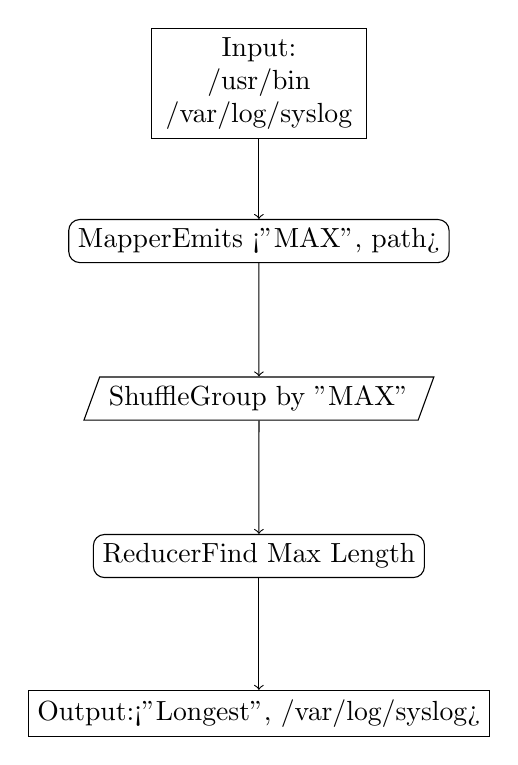
\begin{tikzpicture}[node distance=2cm]
    % Nodes
    \node (input) [rectangle, draw, text width=2.5cm, align=center] {Input:\\ /usr/bin\\ /var/log/syslog};
    \node (map) [rectangle, draw, rounded corners, below of=input] {Mapper\\ Emits <"MAX", path>};
    \node (shuffle) [trapezium, draw, trapezium left angle=70, trapezium right angle=110, below of=map] {Shuffle\\ Group by "MAX"};
    \node (reduce) [rectangle, draw, rounded corners, below of=shuffle] {Reducer\\ Find Max Length};
    \node (output) [rectangle, draw, below of=reduce] {Output:\\ <"Longest", /var/log/syslog>};
    % Arrows
    \draw[->] (input) -- (map);
    \draw[->] (map) -- (shuffle);
    \draw[->] (shuffle) -- (reduce);
    \draw[->] (reduce) -- (output);
\end{tikzpicture}
\caption{MapReduce Flow for Finding the Longest Path}
\end{figure}
\section{Work Distribution}
\begin{itemize}
    \item \textbf{[Member 1 Name]:} Designed the MapReduce C++ abstract class and the core engine logic (shuffling and grouping).
    \item \textbf{[Member 2 Name]:} Implemented the \texttt{LongestPathApp} class, specifically the Mapper logic to route all items to a single key.
    \item \textbf{[Member 3 Name]:} Implemented the Reducer logic to compare string lengths and wrote this LaTeX report.
\end{itemize}
\section{Conclusion}
By forcing all map outputs to share a common key, we effectively centralized the aggregation step. While efficient for this specific "global max" problem, in a truly massive dataset, we would improve this by adding a "Combiner" step to find local maximums before sending data to the Reducer, reducing network traffic.
\end{document}